\documentclass{article}
\usepackage[utf8]{inputenc}
\usepackage{amsmath}
\usepackage{xcolor}
\usepackage[top=2cm, bottom=2cm, left=2cm, right=2cm]{geometry}
\setlength\parindent{0pt}

\usepackage{listings}
%\usepackage{color}
\usepackage{graphicx}
\usepackage{float}
\usepackage{caption}

\usepackage{verbatim}
\let\oldv\verbatim
\let\oldendv\endverbatim

%\userpackage{minted}

\definecolor{dkgreen}{rgb}{0,0.6,0}
\definecolor{gray}{rgb}{0.5,0.5,0.5}
\definecolor{mauve}{rgb}{0.58,0,0.82}
\definecolor{light-gray}{gray}{0.95}


\lstset{frame=tb,
  language=Java,
  aboveskip=6mm,
  belowskip=6mm,
  showstringspaces=false,
  columns=flexible,
  basicstyle={\small\ttfamily},
  numbers=none,
  numberstyle=\tiny\color{gray},
  keywordstyle=\color{blue},
  commentstyle=\color{dkgreen},
  stringstyle=\color{mauve},
  breaklines=true,
  breakatwhitespace=true,
  tabsize=3,
  backgroundcolor=\color{light-gray},
  language=Matlab
}

%\usepackage{natbib} replaced by line below to make refernces work
\usepackage[square,sort,comma,numbers]{natbib}
\usepackage[nottoc,numbib]{tocbibind} %to get references in table of contants
\usepackage{graphicx}

\usepackage{bm}

\usepackage{hyperref}
\hypersetup{
	colorlinks,
	citecolor=black,
	filecolor=black,
	linkcolor=black,
	urlcolor=black
}

\usepackage{mdframed}
\usepackage{lipsum} % for creating dummy text
\mdfdefinestyle{MyFrame}{%
	linecolor=black,	
	backgroundcolor=gray!20!white,
	skipbelow = 8mm,
	skipabove = 8mm}

\usepackage{scrextend}

\usepackage{multimedia}
\usepackage{media9}

\usepackage{booktabs}
\usepackage{adjustbox}

\title{Fys4150\\Project 4 Figures and stuff\\ }
\author{Peter Killingstad and Karl Jacobsen\\
\\
\url{https://github.com/kaaja/fys4150}}

\begin{document}
	
\maketitle



\section*{4b}

\begin{table}[H]
	\centering
	\begin{adjustbox}{width=.5\textwidth}
		\input{/home/karl/doc/subj/att/fys4150p/proj4/resultsKeep/Out4b4Rport.txt}%
	\end{adjustbox}
	\caption{Estimated quantitites \\ \textit{.}}
	\label{1}
\end{table}

\begin{table}[H]
	\centering
	\begin{adjustbox}{width=.5\textwidth}
		\input{/home/karl/doc/subj/att/fys4150p/proj4/resultsKeep/Out4b4RportDev.txt}%
	\end{adjustbox}
	\caption{Percentage deviations from analytical results}
	\label{1}
\end{table}


\section{4c}

\begin{minipage}{.45\textwidth} 
	\begin{figure}[H]
		\centering
		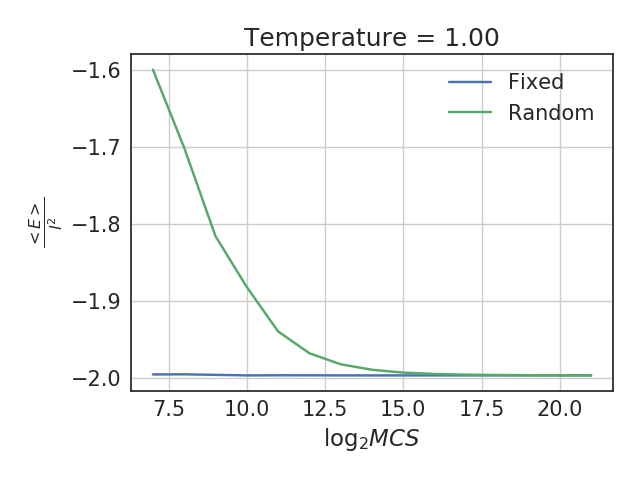
\includegraphics[width=0.99\textwidth]{/home/karl/doc/subj/att/fys4150/project4/resultsKeep/4cEnergy1.png}
		\caption{Expected Energy divided by $L^2$. $T=1.0$. \\ \textit{Equilibrium reached after $2^{20}$ Monte Carlo cycles.}}
		\label{1}
	\end{figure}
\end{minipage}\hfill
\begin{minipage}{.45\textwidth} 
	\begin{figure}[H]
		\centering
		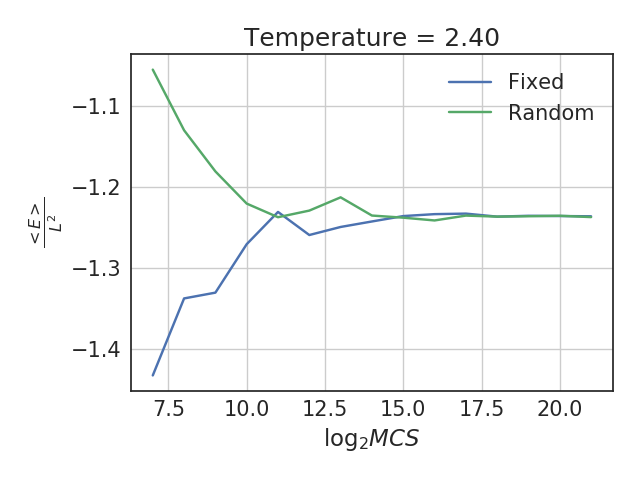
\includegraphics[width=0.99\textwidth]{/home/karl/doc/subj/att/fys4150/project4/resultsKeep/4cEnergy24.png}
		\caption{Expected Energy divided by $L^2$. $T = 2.4$. \\ \textit{Equilibrium reached at same point as for $T=1$}.}
		\label{1}
	\end{figure}
\end{minipage}\hfill
\vspace{2ex}

\begin{minipage}{.45\textwidth} 
	\begin{figure}[H]
		\centering
		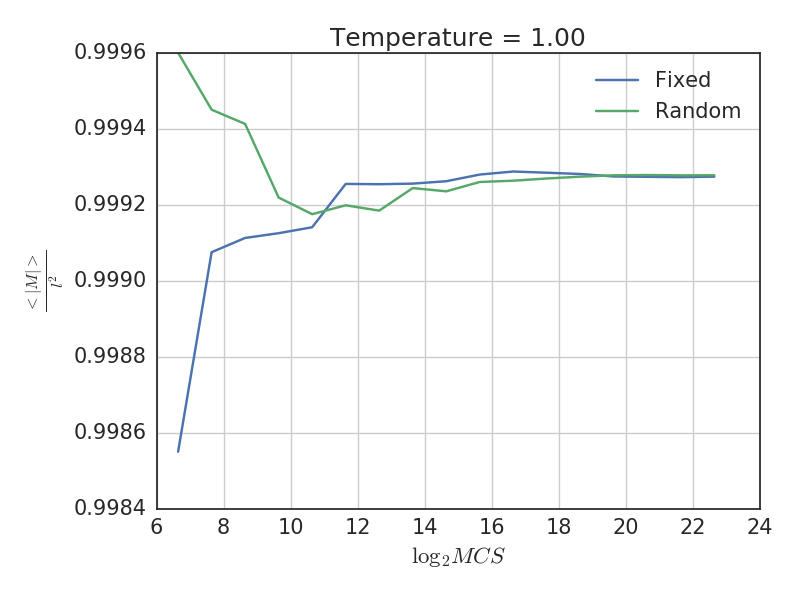
\includegraphics[width=0.99\textwidth]{/home/karl/doc/subj/att/fys4150/project4/resultsKeep/4cMoment1.png}
		\caption{Expected absolute magnetic momentum divided by $L^2$. $T = 1.0$. \\ \textit{Equilibrium reached at same point as for the energy.}}
		\label{1}
	\end{figure}
\end{minipage}\hfill
\begin{minipage}{.45\textwidth} 
	\begin{figure}[H]
		\centering
		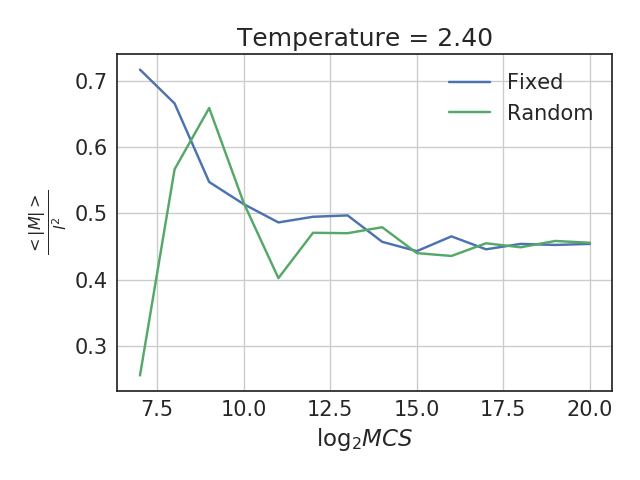
\includegraphics[width=0.99\textwidth]{/home/karl/doc/subj/att/fys4150/project4/resultsKeep/4cMoment24.png}
		\caption{Expected absolute magnetic momentum divided by $L^2$. $T = 2.4$. \\ \textit{Equilibrium reached at same point as for the others.}}
		\label{1}
	\end{figure}
\end{minipage}\hfill
\vspace{2ex}

\begin{figure}[H]
	\centering
	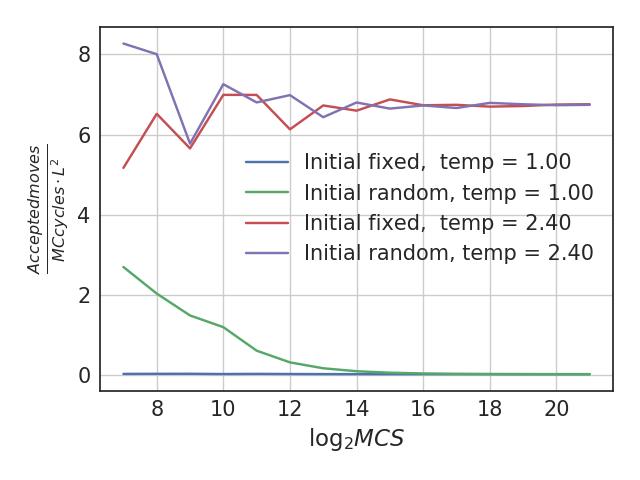
\includegraphics[width=0.6\textwidth]{/home/karl/doc/subj/att/fys4150/project4/resultsKeep/4cAcceptedMoves.png}
	\caption{Accepted moved divided by $L^2$. \\ \textit{}}
	\label{1}
\end{figure}

\section{4d}


\begin{table}[H]
	\centering
	\begin{adjustbox}{width=1\textwidth}
		\input{/home/karl/doc/subj/att/fys4150/project4/resultsKeep/4dTableFixed.txt}%
	\end{adjustbox}
	\caption{Statistics. Fixed initial config. \\ \textit{.}}
	\label{1}
\end{table}

\begin{table}[H]
	\centering
	\begin{adjustbox}{width=1\textwidth}
		\input{/home/karl/doc/subj/att/fys4150/project4/resultsKeep/4dTableRandom.txt}%
	\end{adjustbox}
	\caption{Statistics. Random initial config. \\ \textit{.}}
	\label{1}
\end{table}



\begin{minipage}{.45\textwidth} 
	\begin{figure}[H]
		\centering
		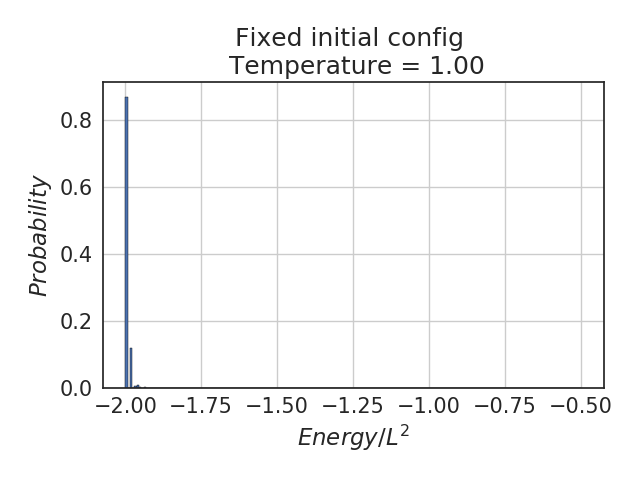
\includegraphics[width=0.99\textwidth]{/home/karl/doc/subj/att/fys4150/project4/resultsKeep/4dHistogramFixed1.png}
		\caption{Probability distribution. Fixed intital $T = 1$. \\ \textit{}}
		\label{1}
	\end{figure}
\end{minipage}\hfill
\begin{minipage}{.45\textwidth} 
	\begin{figure}[H]
		\centering
		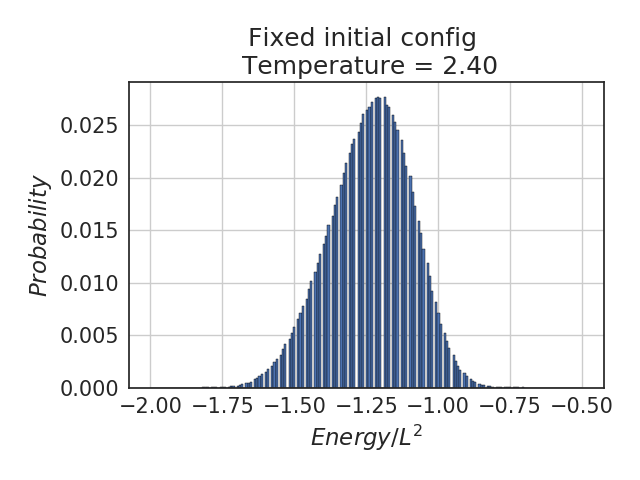
\includegraphics[width=0.99\textwidth]{/home/karl/doc/subj/att/fys4150/project4/resultsKeep/4dHistogramFixed24.png}
		\caption{Probability distribution. Fixed intital $T = 2.4$.. \\ \textit{}.}
		\label{1}
	\end{figure}
\end{minipage}\hfill
\vspace{2ex}

\begin{minipage}{.45\textwidth} 
	\begin{figure}[H]
		\centering
		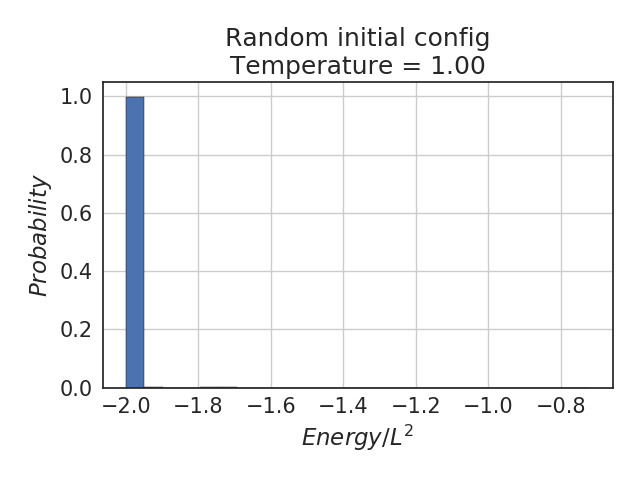
\includegraphics[width=0.99\textwidth]{/home/karl/doc/subj/att/fys4150/project4/resultsKeep/4dHistogramRandom1.png}
		\caption{Probability distribution. Random intital $T = 1$. \\ \textit{}}
		\label{1}
	\end{figure}
\end{minipage}\hfill
\begin{minipage}{.45\textwidth} 
	\begin{figure}[H]
		\centering
		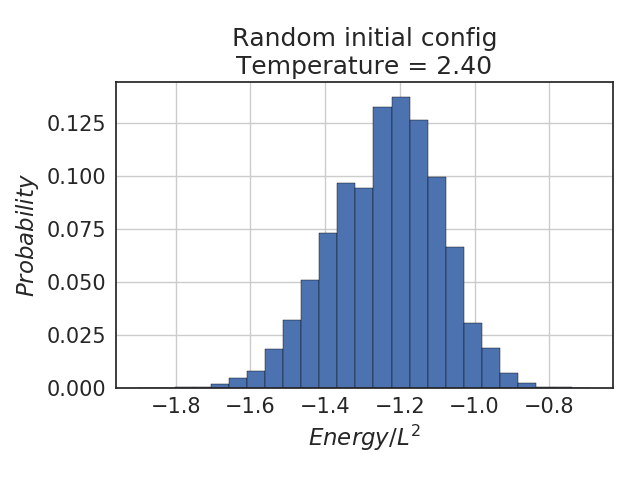
\includegraphics[width=0.99\textwidth]{/home/karl/doc/subj/att/fys4150/project4/resultsKeep/4dHistogramRandom24.png}
		\caption{Probability distribution. Random intital $T = 2.4$.  \\ \textit{}}
		\label{1}
	\end{figure}
\end{minipage}\hfill
\vspace{2ex}



\section{4e}

\begin{minipage}{.45\textwidth} 
	\begin{figure}[H]
		\centering
		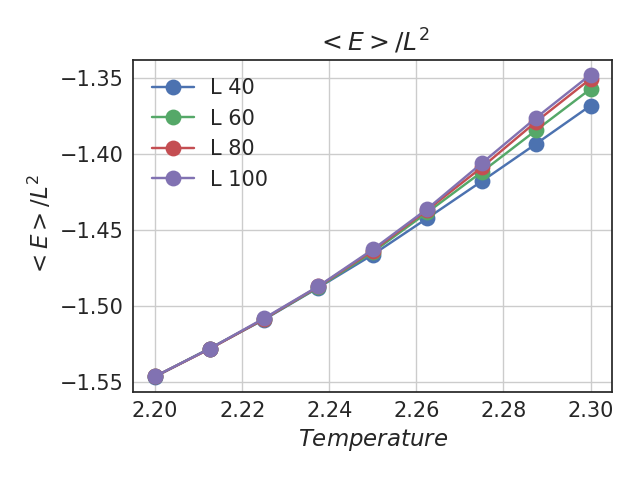
\includegraphics[width=0.99\textwidth]{/home/karl/doc/subj/att/fys4150/project4/resultsKeep/4eEavg.png}
		\caption{Expected value energy. \\ \textit{}}
		\label{1}
	\end{figure}
\end{minipage}\hfill
\begin{minipage}{.45\textwidth} 
	\begin{figure}[H]
		\centering
		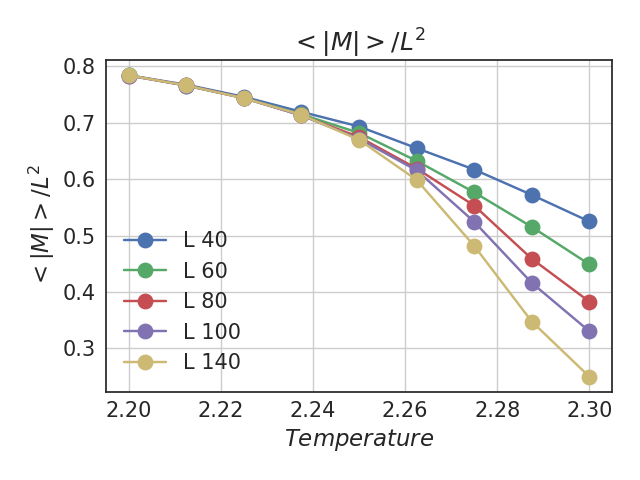
\includegraphics[width=0.99\textwidth]{/home/karl/doc/subj/att/fys4150/project4/resultsKeep/4eabsMavg.png}
		\caption{Expected value magnetic moment.\\ \textit{}.}
		\label{1}
	\end{figure}
\end{minipage}\hfill
\vspace{2ex}

\begin{minipage}{.45\textwidth} 
	\begin{figure}[H]
		\centering
		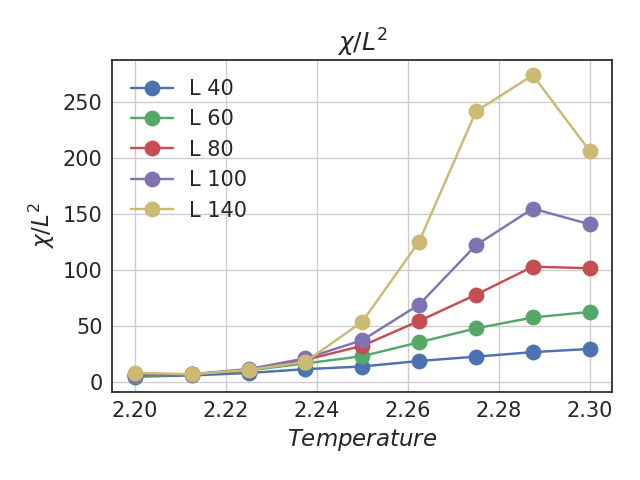
\includegraphics[width=0.99\textwidth]{/home/karl/doc/subj/att/fys4150/project4/resultsKeep/4echi.png}
		\caption{Susceptibility\\ \textit{}}
		\label{1}
	\end{figure}
\end{minipage}\hfill
\begin{minipage}{.45\textwidth} 
	\begin{figure}[H]
		\centering
		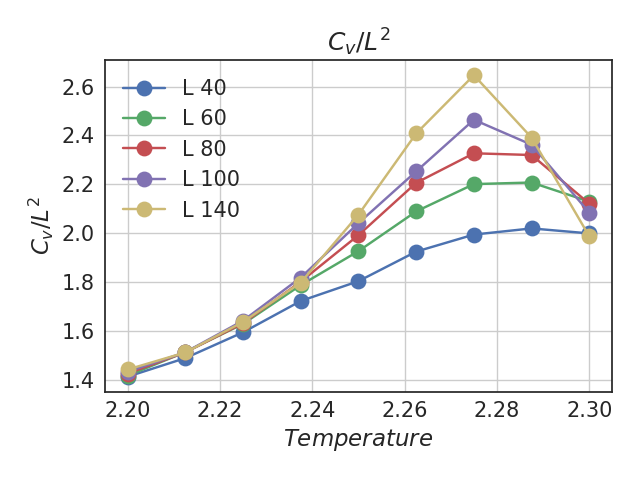
\includegraphics[width=0.99\textwidth]{/home/karl/doc/subj/att/fys4150/project4/resultsKeep/4eCv.png}
		\caption{Specific heat capacity\\ \textit{}}
		\label{1}
	\end{figure}
\end{minipage}\hfill
\vspace{2ex}


\begin{table}[H]
	\centering
	\begin{adjustbox}{width=.5\textwidth}
		\input{/home/karl/doc/subj/att/fys4150/project4/resultsKeep/Out4eTcCritical.txt}%
	\end{adjustbox}
	\caption{Estimated $T_C$. \\ \textit{.}}
	\label{1}
\end{table}



\end{document}
